% !TEX root = ../dissertation.tex
\chapter{Dumbbell Spacecraft about an asteroid}
\section[Moment of Inertia]{Moment of Inertia derivation}\label{sec:moi_derivation}
The inertia tensor for a continuous body is given by
\begin{align}\label{eq:moi_hatmap}
    J_I = \int_\mathcal{B} S(\vecbf{\rho})^T S(\vecbf{\rho}) \, dm ,
\end{align}
where \( \vecbf{\rho}\) defines the position of the mass element \( dm \) relative to a body-fixed reference frame located at the center of mass of \( \mathcal{B} \) and aligned with the principle axes.
The hat map identity
\begin{align*}
    S(\vecbf{\rho})^T S(\vb{\rho}) &= (\vb{\rho}^T\vb{\rho}) I - \vb{\rho}\vb{\rho}^T , \\
    &= \tr{\vb{\rho}\vb{\rho}^T} I - \vb{\rho}\vb{\rho}^T ,
\end{align*}
is used to equivalently define~\cref{eq:moi_hatmap} in a more familar form as
\begin{align}\label{eq:moi}
    J_I = \int_{\mathcal{B}} \bracket{\tr{\vb{\rho}\vb{\rho}^T} I - \vb{\rho}\vb{\rho}^T} \, dm .
\end{align}

The dumbbell model of the spacecraft is shown in~\cref{fig:dumbbell_sc}.
\begin{figure}
    \centering
    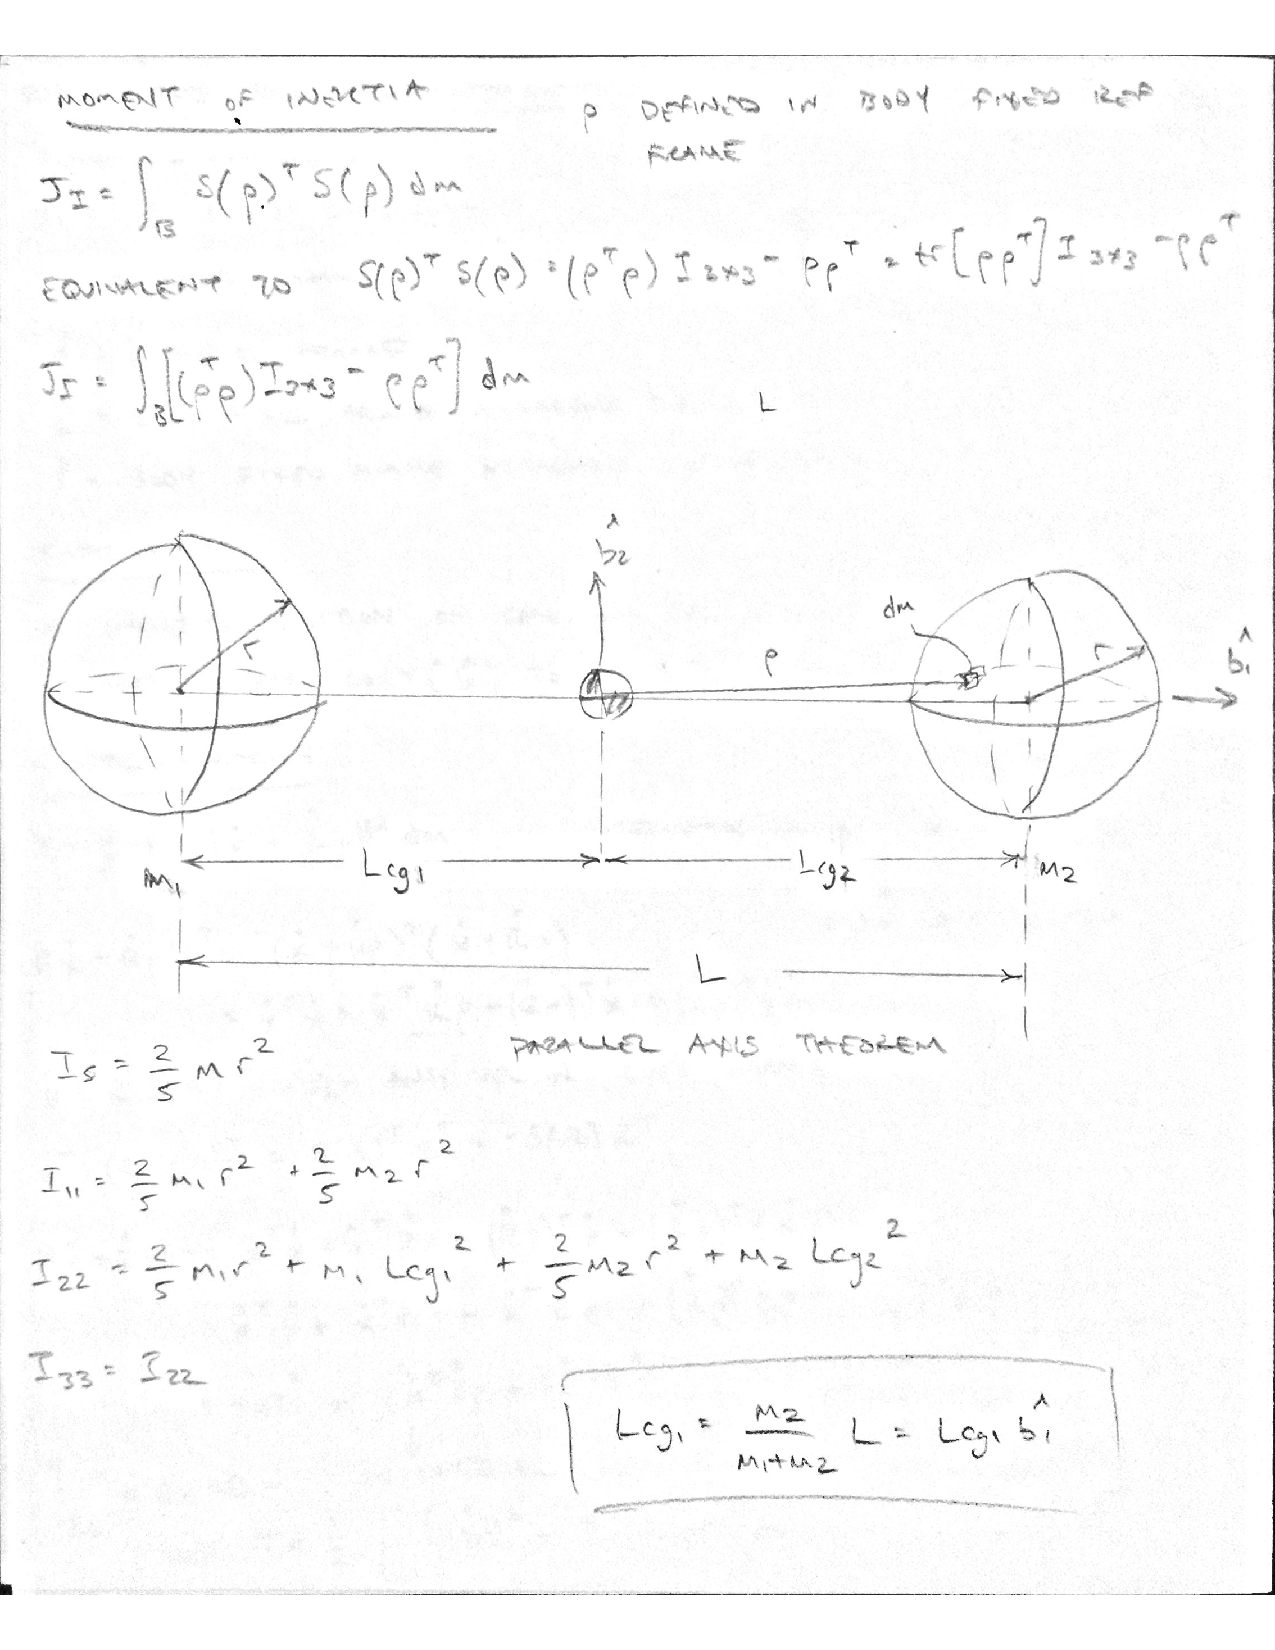
\includegraphics[width=0.5\textwidth]{figures/dumbbell_model.pdf}
    \caption{Dumbbell Spacecraft Model (REPLACE WITH TIKZ)\label{fig:dumbbell_sc}}
\end{figure}
The model is composed of two solid spherical masses connected by a massless rod of length \( l\). 
The body fixed reference frame vector, \( \vh{b}_1\), is aligned with the connecting rod and points along the direction of the body from \( m_1 \) to \( m_2\).
As a result, the position of \( m_2 \) with respect to \( m_1\) is \( \vb{r}_{12} = l \vh{b}_1\).
The center of mass of the dumbbell, defined with respect to \( m_1\), is computed as
\begin{align}\label{eqn:com}
    \vb{r}_{2c} &= \frac{1}{\sum_i m_i} \sum_i m_i \parenth{\vb{r}_i - \vb{r}_1},\\
    &= \frac{m_2}{m_1+m_2} l \vh{b}_1 , \\
    &= l_{cg_{1}} \vh{b}_1 .
\end{align}

Since the mass of the model is concentrated in the two spherical masses,~\cref{eq:moi} is redefined as
\begin{align*}
    J_i = \sum_i^2 \int_{\mathcal{B}} \bracket{\tr{\vb{\rho}_i\vb{\rho}_i^T} I - \vb{\rho}_i \vb{\rho}_i^T} \, dm ,
\end{align*}
where \( \vb{\rho}_i = \vb{\zeta}_i + \vb{\eta}_i \) with \( \vb{\zeta}_i \) defining the center of each spherical mass and \( \vb{\eta}_i \) the location of \( dm \) relative to the center of each sphere.
Using this, the integral term can be expanded as
\begin{align*}
    \bracket{\tr{\vb{\rho}_i\vb{\rho}_i^T} I - \vb{\rho}_i \vb{\rho}_i^T} &= \parenth{\vb{\zeta}_i + \vb{\eta}_i}^T \parenth{\vb{\zeta}_i + \vb{\eta}_i}^T I - \parenth{\vb{\zeta}_i + \vb{\eta}_i} \parenth{\vb{\zeta}_i + \vb{\eta}_i}^T , \\
    &= \parenth{\vb{\zeta}_i^T \vb{\zeta}_i + \vb{\zeta}_i \vb{\eta}_i + \vb{\eta}_i^T \vb{\zeta}_i + \vb{\eta}_i^T \vb{\eta}_i} I - \vb{\zeta}_i \vb{\zeta}_i^T - \vb{\zeta}_i \vb{\eta}_i^T - \vb{\eta}_i \vb{\zeta}_i^T - \vb{\eta}_i \vb{\eta}_i^T .
\end{align*}
From the definition of the center of mass, \( \int_{\mathcal{B}_i} \vb{\eta}_i \, dm = 0\), the integral becomes
\begin{align*}
    J_I &= \sum_i \int_{\mathcal{B}_i} \parenth{ \vb{\zeta}_i^T \vb{\zeta}_i I - \vb{\zeta}_i \vb{\zeta}_i^T} + \parenth{\vb{\eta}_i^T \vb{\eta}_i I - \vb{\eta}_i \vb{\eta}_i^T} + \parenth{2 \vb{\zeta}_i^T \vb{\eta}_i I - \vb{\zeta}_i \vb{\eta}_i^T - \vb{\eta}_i \vb{\zeta}_i^T} \, dm , \\
    &= \sum_i \int_{\mathcal{B}_i} \parenth{ \vb{\zeta}_i^T \vb{\zeta}_i I - \vb{\zeta}_i \vb{\zeta}_i^T} + \parenth{\vb{\eta}_i^T \vb{\eta}_i I - \vb{\eta}_i \vb{\eta}_i^T} \, dm , \\
    &= \sum_i \int_{\mathcal{B}_i} \parenth{ \vb{\zeta}_i^T \vb{\zeta}_i I - \vb{\zeta}_i \vb{\zeta}_i^T} \, dm + \int_{\mathcal{B}_i}\parenth{\vb{\eta}_i^T \vb{\eta}_i I - \vb{\eta}_i \vb{\eta}_i^T} \, dm , \\
    &= \sum_i m_i \parenth{ \vb{\zeta}_i^T \vb{\zeta}_i I - \vb{\zeta}_i \vb{\zeta}_i^T} + J_i
\end{align*}
The moment of inertia of each sphere is \( J_i \) and easily computed to be
\begin{align*}
    J_i = \text{diag} \begin{bmatrix} \frac{2}{5} m_i r_i^2 & \frac{2}{5} m_i r_i^2 & \frac{2}{5} m_i r_i^2\end{bmatrix}.
\end{align*}
The location of the center of each sphere is 
\begin{align}
    \vb{\zeta}_1 &= -l_{cg_{1}} \vh{b}_1 , \\
    \vb{\zeta}_2 &= \parenth{l - l_{cg_{1}}} \vh{b}_1.
\end{align}
Using this gives the final moment of inertia tensor as
\begin{align}
    J_I = \begin{bmatrix}
        \frac{2}{5} m_1 r_1^2 + \frac{2}{5} m_2 r_2^2  & 0 & 0 \\
        0 & \frac{2}{5} m_1 r_1^2 + \frac{2}{5} m_2 r_2^2 + m_1 l_1^2 + m_2 l_2^2 & 0 \\
        0 & 0 & \frac{2}{5} m_1 r_1^2 + \frac{2}{5} m_2 r_2^2 + m_1 l_1^2 + m_2 l_2^2
    \end{bmatrix} .
\end{align}
We define \( J_d \) as the non-standard moment of inertia.
It is related to the standard moment of inertia tensor, \( J_I\), through the following relationship
\begin{align}\label{eq:nonstandard_moi}
    J_I &= \int_{\mathcal{B}} S(\vb{\rho})^T S(\vb{\rho}) \, dm \nonumber \\
    &= \int_{\mathcal{B}} \vb{\rho}^T \vb{\rho} I - \vb{\rho}\vb{\rho}^T \, dm , \nonumber \\
    &= \int_{\mathcal{B}} \tr{\vb{\rho} \vb{\rho}^T} I - \vb{\rho}\vb{\rho}^T \, dm \nonumber \\
    &= \tr{\int_{\mathcal{B}} \vb{\rho} \vb{\rho}^T \, dm} I - \int_{\mathcal{B}} \vb{\rho} \vb{\rho}^T \, dm , \nonumber \\
    &= \tr{J_d} I - J_d .
\end{align}
Using the previous definition for \( \vb{\rho}_i \) we can expand this further as
\begin{align}
    J_d &= \sum_i \int_{B_i} \parenth{\vb{\zeta}_i + \vb{\eta}_i}^T \parenth{\vb{\zeta}_i + \vb{\eta}_i} \, dm \, \\
    &= \sum_i \int_{B_i} \vb{\zeta}_i \vb{\zeta}_i^T + \vb{\eta}_i \vb{\eta}_i^T \, dm , \\
    &= \sum_i m_i \vb{\zeta}_i \vb{\zeta}_i^T + \frac{1}{5}m_i r_i^2 .
\end{align}

\section{Inertial Frame Derivation}\label{sec:asteroid_inertial_eoms}

There are three frames of interest for our problem:
\begin{itemize}
    \item \( \hat{\vecbf{e}}_i \) - Inertial frame that is fixed at the center of the asteroid
    \item \( \hat{\vecbf{b}}_i \) - Dumbbell body fixed frame located at the center of mass of the dumbbell and aligned with the principal axes
    \item \( \hat{\vecbf{f}}_i \) - Asteroid body fixed frame located at the center of mass of the asteroid and aligned with the principal axes
\end{itemize}
We assume that the motion of the asteroid is not affected by the presence of the dumbbell spacecraft.
This is also called the restricted two body problem.
The kinematics of the dumbbell and asteroid are described in the inertial frame by
\begin{itemize}
    \item \( \vecbf{x} \) - the position of the center of mass of the dumbbell spacecraft represented in the inertial frame \( \vecbf{e}_i\)
    \item \( R \) - the rotation matrix which transforms vectors defined in the spacecraft fixed frame, \( \vecbf{b}_i \), to the inertial frame, \( \vecbf{e}_i \)
    \item \( \vecbf{\Omega} \) - the angular velocity of the spacecraft body fixed frame relative to the inertial frame and represented in the dumbell body fixed frame \( \vecbf{b}_i \)
    \item \( R_A \) - the rotation matrix which transforms vectors defined in the asteroid fixed frame, \( \vecbf{f}_i \), to the inertial frame, \( \vecbf{e}_i \)
\end{itemize}

\subsection{Kinetic Energy}
The kinetic energy of the dumbbell can be defined as
\begin{align}
    T = \frac{1}{2} \int_{\mathsf{B}} \norm{\dot{\vecbf{x}} + \dot{R} \vecbf{\rho} }^2 \, dm ,
\end{align}
where the vector \( \vecbf{\rho} \) is defined in the dumbbell body fixed frame, \( \hat{\vecbf{b}}_i \) and represents the position of the mass element \( dm \) relative to the center of mass.
The quadratic term \( \norm{\dot{\vecbf{x}} + \dot{R} \vecbf{\rho} }^2 \) is expanded as
\begin{align}
    \norm{\dot{\vecbf{x}} + \dot{R} \vecbf{\rho} }^2 &= \dot{\vecbf{x}}^T \dot{\vecbf{x}} + \dot{\vecbf{x}}^T \dot{R} \vecbf{\rho} + \parenth{ \dot{R} \vecbf{\rho}}^T \dot{\vecbf{x}} + \parenth{\dot{R} \vecbf{\rho}}^T \parenth{\dot{R} \vecbf{\rho}} \nonumber\\
    &= \dot{\vecbf{x}}^T \dot{\vecbf{x}} + 2 \dot{\vecbf{x}}^T \dot{R} \vecbf{\rho} + \parenth{\dot{R} \vecbf{\rho}}^T \parenth{\dot{R} \vecbf{\rho}} \nonumber\\
    &= \norm{\dot{\vecbf{x}}}^2 + 2 \dot{\vecbf{x}}^T \dot{R} \vecbf{\rho} + \norm{\parenth{\dot{R} \vecbf{\rho}} }^2 .
\end{align}
The second term will go to zero from the definition of the center of mass
\begin{align}
    \int_{\mathsf{B}} \vecbf{\rho} \, dm = 0 .
\end{align}
Combining this with the kinematic equations of motion, \( \dot{R} = R S(\vecbf{\Omega}) \), gives
\begin{align}
    T &= \frac{1}{2} \int_{\mathsf{B}} \braces{ \norm{\dot{\vecbf{x}}}^2 + \norm{\parenth{\dot{R} \vecbf{\rho}} }^2  } \, dm \nonumber\\
    &= \frac{1}{2} \int_{\mathsf{B}} \braces{ \norm{\dot{\vecbf{x}}}^2 + \parenth{\dot{R} \vecbf{\rho}}^T \parenth{\dot{R} \vecbf{\rho}}  } \, dm \nonumber\\
    &= \frac{1}{2} \int_{\mathsf{B}} \braces{ \norm{\dot{\vecbf{x}}}^2 + \vecbf{\rho}^T S(\vecbf{\Omega})^T R^T R S(\vecbf{\Omega}) \vecbf{\rho}  } \, dm \nonumber\\
    &= \frac{1}{2} \int_{\mathsf{B}} \braces{ \norm{\dot{\vecbf{x}}}^2 + \norm{S(\vecbf{\Omega}) \vecbf{\rho}}^2  } \, dm  .
\end{align}

The first term is simplified as
\begin{align*}
    \int_{\mathcal{B}} \norm{\dot{\vb{x}}}^2 \, dm = m \norm{\vb{x}}^2 .
\end{align*}
We use the trace property
\begin{align*}
    \norm{\vb{x}^2} = \vb{x}^T \vb{x} = \tr{\vb{x} \vb{x}^T} .
\end{align*}
Using this property, the second term becomes
\begin{align*}
    \int_{\mathcal{B}} \norm{S(\vb{\Omega}) \vb{\rho}}^2 \, dm &= \int_{\mathcal{B}} \parenth{S(\vb{\Omega}) \vb{\rho}}^T \parenth{S(\vb{\Omega}) \vb{\rho}}\, dm , \\
    &= \int_{\mathcal{B}} \tr{S(\vb{\Omega}) \vb{\rho} \vb{\rho}^T S(\vb{\Omega})^T}\, dm , \\
    &= \tr{S(\vb{\Omega}) \bracket{\int_{\mathcal{B}} \vb{\rho} \vb{\rho}^T \, dm} S(\vb{\Omega})^T} , \\
    &= \tr{S(\vb{\Omega}) J_d S(\vb{\Omega})^T} .
\end{align*}

Finally, the kinetic energy of the dumbbell is defined as
\begin{align}\label{eq:kinetic_energy}
    T = \frac{1}{2} m \norm{\dot{\vb{x}}}^2 + \frac{1}{2} \tr{S(\vb{\Omega}) J_d S(\vb{\Omega})^T} .
\end{align}

\subsection{Gravitational Potential Energy}\label{ssec:potential_energy}

\subsubsection{Polyhedron Gravity Model}\label{sec:polyhedron_model}

We represent the gravitational potential of the asteroid using a polyhedron gravitation model.
This model is composed of a polyhedron, which is a three-dimensional solid body, that is defined by a series of vectors in the body-fixed frame.
The vectors define vertices in the body-fixed frame as well as planar faces which compose the surface of the asteroid.
We assume that each face is a triangle composed of three vertices and three edges.
As a result, only two faces meet at each edge while three faces meet at each vertex.
Only the body-fixed vectors, and their associated topology, is required to define the exterior gravitational model.
References~\cite{werner1994} and~\cite{werner1996} give a detailed derivation of the polyhedron model.
Here, we summarize the key developments and equations required for implementation.

Consider three vectors \( \vecbf{v}_1, \vecbf{v}_2, \vecbf{v}_3 \in \R^{3 \times 1} \), assumed to be defined in the asteroid body-fixed frame and are ordered in a counterclockwise direction about an outward facing normal vector, which define a face.
It is easy to define the three edges of each face as
\begin{align}\label{eq:edges}
    \vecbf{e}_{i+1,i} = \vecbf{v}_{i+1} - \vecbf{v}_i \in \R^{3 \times 1 },
\end{align}
where the index \( i \in \parenth{1,2,3} \) is used to permute all edges of each face.
Since each edge is a member of two faces, there exist two edges which are defined in opposite directions between the same vertices.
We can also define the outward normal vector to face \( f\)  as
\begin{align}\label{eq:face_normal}
    {\vecbf{n}}_f &= \parenth{\vecbf{v}_{2} - \vecbf{v}_1} \times \parenth{\vecbf{v}_{3} - \vecbf{v}_2} \in \R^{3 \times 1},
\end{align}
and the outward facing normal vector to each edge as
\begin{align}\label{eq:edge_normal}
    {\vecbf{n}}_{i+1,i}^f &= \parenth{\vecbf{v}_{i+1} - \vecbf{v}_i} \times {\vecbf{n}}_f \in \R^{3 \times 1}.
\end{align}
For each face we define the face dyad \( \vecbf{F}_f \) as
\begin{align}\label{eq:face_dyad}
    \vecbf{F}_f &= {\vecbf{n}}_f {\vecbf{n}}_f \in \R^{3 \times 3}.
\end{align}
Each edge is a member of two faces and has an outward pointing edge normal vector, given in~\cref{eq:edge_normal}, perpendicular to both the edge and the face normal.
For the edge connecting the vectors \( \vecbf{v}_1 \) and \( \vecbf{v}_2 \), which are shared between the faces \(A\) and \( B\), the per edge dyad is given by
\begin{align}\label{eq:edge_dyad}
    \vecbf{E}_{12} = {\vecbf{n}}_A {\vecbf{n}}_{12}^A + {\vecbf{n}}_B {\vecbf{n}}_{21}^B \in \R^{3 \times 3}.
\end{align}
The edge dyad \( \vecbf{E}_e  \), is defined for each edge and is a function of the two adjacent faces meeting at that edge.
The face dyad \( \vecbf{F}_f \), is defined for each face and is a function of the face normal vectors.

Let \( \vecbf{r}_i \in \R^{3 \times 1} \) be the vector from the spacecraft to the vertex \( \vecbf{v}_i \), defined in the asteroid body fixed frame, and it's length is given by \( r_i = \norm{\vecbf{r}_i} \in \R^{1} \).
The per-edge factor \( L_e \in \R^{1}\), for the edge connecting vertices \( \vecbf{v}_i \) and \( \vecbf{v}_j \), with a constant length \( e_{ij} = \norm{\vecbf{e}_{ij}} \in \R^1\) is
\begin{align}\label{eq:edge_factor}
    L_e &= \ln \frac{r_i + r_j + e_{ij}}{r_i + r_j - e_{ij}}.
\end{align}
For the face defined by the vertices \( \vecbf{v}_i, \vecbf{v}_j, \vecbf{v}_k \) the per-face factor \( \omega_f \in \R^{1} \) is
\begin{align}\label{eq:face_factor}
    \omega_f &= 2 \arctan \frac{\vecbf{r}_i \cdot \vecbf{r}_j \times \vecbf{r}_k}{r_i r_j r_k + r_i \parenth{\vecbf{r}_j \cdot \vecbf{r}_k} + r_j \parenth{\vecbf{r}_k \cdot \vecbf{r}_i} + r_k \parenth{\vecbf{r}_i \cdot \vecbf{r}_j}} .
\end{align}
The gravitational potential due to a constant density polyhedron is given as
\begin{align}\label{eq:potential}
    U(\vecbf{r}) &= \frac{1}{2} G \sigma \sum_{e \in \text{edges}} \vecbf{r}_e \cdot \vecbf{E}_e \cdot \vecbf{r}_e \cdot L_e - \frac{1}{2}G \sigma \sum_{f \in \text{faces}} \vecbf{r}_f \cdot \vecbf{F}_f \cdot \vecbf{r}_f \cdot \omega_f \in \R^1,
\end{align}
where \( \vecbf{r}_e\) and \(\vecbf{r}_f \) are the vectors from the spacecraft to any point on the respective edge or face, \( G\) is the universal gravitational constant, and \( \sigma \) is the constant density of the asteroid.
Furthermore we can use these definitions to define the attraction, gravity gradient matrix, and Laplacian as
\begin{align}
    \nabla U ( \vecbf{r} ) &= -G \sigma \sum_{e \in \text{edges}} \vecbf{E}_e \cdot \vecbf{r}_e \cdot L_e + G \sigma \sum_{f \in \text{faces}} \vecbf{F}_f \cdot \vecbf{r}_f \cdot \omega_f \in \R^{3 \times 1} , \label{eq:attraction}\\
    \nabla \nabla U ( \vecbf{r} ) &= G \sigma \sum_{e \in \text{edges}} \vecbf{E}_e  \cdot L_e - G \sigma \sum_{f \in \text{faces}} \vecbf{F}_f \cdot \omega_f \in \R^{3 \times 3}, \label{eq:gradient_matrix}\\
    \nabla^2 U &= -G \sigma \sum_{f \in \text{faces}}  \omega_f \in \R^1 .\label{eq:laplacian}
\end{align}

One interesting thing to note is that both~\cref{eq:face_dyad,eq:edge_dyad} can be precomputed without knowledge of the position of the satellite.
They are both solely functions of the vertices and edges of the polyhedral shape model and are computed once and stored.
Once a position vector \( \vecbf{r} \) is defined, the scalars given in~\cref{eq:edge_factor,eq:face_factor} can be computed for each face and edge.
Finally,~\cref{eq:potential} is used to compute the gravitational potential on the spacecraft.
The Laplacian, defined in~\cref{eq:laplacian}, gives a simple method to determine if the spacecraft has collided with the body~\cite{werner1996}. 

\subsection{Potential Energy}
The potential energy of the system is a function of the attraction due to gravity from~\cref{sec:polyhedron_model}.
The potential energy of the dumbbell is then defined as
\begin{align}\label{eq:potential_energy}
    V( \vecbf{x}, R ) =  - m_1 U \parenth{R_A^T \parenth{\vecbf{x} + R \vecbf{\rho}_1}} - m_2 U \parenth{R_A^T \parenth{\vecbf{x} + R \vecbf{\rho}_2}} .
\end{align}
Since, the potential model is defined in the asteroid fixed frame, we need to transform the position vectors from the inertial frame to the asteroid body frame.

\subsection{Variation}
The Lagrangian is given as the difference between~\cref{eq:kinetic_energy} and~\cref{eq:potential_energy}
\begin{align}\label{eq:lagrangian}
    L = \frac{1}{2} m \norm{\dot{\vb{x}}}^2 + \frac{1}{2} \tr{S(\vb{\Omega}) J_d S(\vb{\Omega})^T} + m_1 U \parenth{R_A^T \parenth{\vecbf{x} + R \vecbf{\rho}_1}} + m_2 U \parenth{R_A^T \parenth{\vecbf{x} + R \vecbf{\rho}_2}} .
\end{align}
The equations of motion can be defined by determining the variation of the Lagrangian, \( \delta L\).
\subsection{Potential Energy Variation}

\subsection{Kinetic Energy Variation}


\subsubsection{Hamilton's Principle}

\subsection[Inertial EOMs]{Inertial equations of motion}\label{sec:inertial_eoms}

The inertial equations of motion are defined as
\begin{align}
    \dot{\vb{x}} &= \vb{v}, \\
    \parenth{m_1 + m_2} \dot{\vecbf{v}} &= m_1 R_A \deriv{U}{\vecbf{z}_1} + m_2 R_A \deriv{U}{\vecbf{z}_2}, \\
    \dot{R} &= R S(\vb{\Omega}) , \\
    J \dot{\vecbf{\Omega}} + \vecbf{\Omega} \times J \vecbf{\Omega} &= \vecbf{M}_1 + \vecbf{M}_2.
\end{align}
The vectors \( \vecbf{z}_1 \) and \( \vecbf{z}_2\) define the position of the dumbbell masses as represented in the asteroid fixed frame and are defined as
\begin{align}
    \vecbf{z}_1 &= R_A^T \parenth{\vecbf{x} + R \vecbf{\rho}_1} , \\
    \vecbf{z}_2 &= R_A^T \parenth{\vecbf{x} + R \vecbf{\rho}_2}.
\end{align}
The moment on the dumbbell \( \vecbf{M}_i\) is defined as
\begin{align}
    \vecbf{M}_i = m_i \parenth{S(R_A^T \vb{\rho}_i) R^T \deriv{U}{\vb{z}_i}}, 
\end{align}
where \( \vb{\rho}_i \) defines the position of each mass in the dumbbell fixed frame.

\subsection{Simulation verification}\label{ssec:inertial_eoms_sim}
To verify the inertial equations of motion, a long duration simulation is performed and the total energy of the dumbbell is computed.
In this case, it is assumed that the asteroid 4769 Castalia is modeled using \num{256} faces.
The dumbbell is defined with the following properties:
\begin{align*}
    m_1 &= m_2 = \SI{100}{\kilo\gram},  \quad l = \SI{3}{\meter} ,\\
    r_1 &= r_2 = \SI{1}{\meter}.
\end{align*} 
The dumbbell begins with the initial state defined as
\begin{align*}
    \vb{x}_0 &= \begin{bmatrix} 1.495746722510590 & 0.000001002669660 & 0.006129720493607\end{bmatrix}^T , \\
    \dot{\vb{x}}_0 &= \begin{bmatrix} 0.000000302161724 & -0.000899607989820 & -0.000000013286327\end{bmatrix} + \hat\omega \vb{x}_0 , \\
    R_0 & = I , \\
    \vb{\Omega}_0 &= \begin{bmatrix} 0 & 0 & 0\end{bmatrix}^T.
\end{align*}
The motion of the dumbbell is simulated over \SI{1e6}{\second} with a step size of \SI{1}{\second} using the numerical integration routine \texttt{scipy.odeint} which uses the FORTRAN library \texttt{odepack}.
The kinetic and potential energy of the dumbbell are computed using~\cref{eq:kinetic_energy,eq:potential_energy} and plotted over the entire timespan.
\Cref{fig:inertial_energy} shows the history of the energy over the simulation.
We can see that total energy remains well behaved over the long simulation.
\begin{figure}
    \centering
    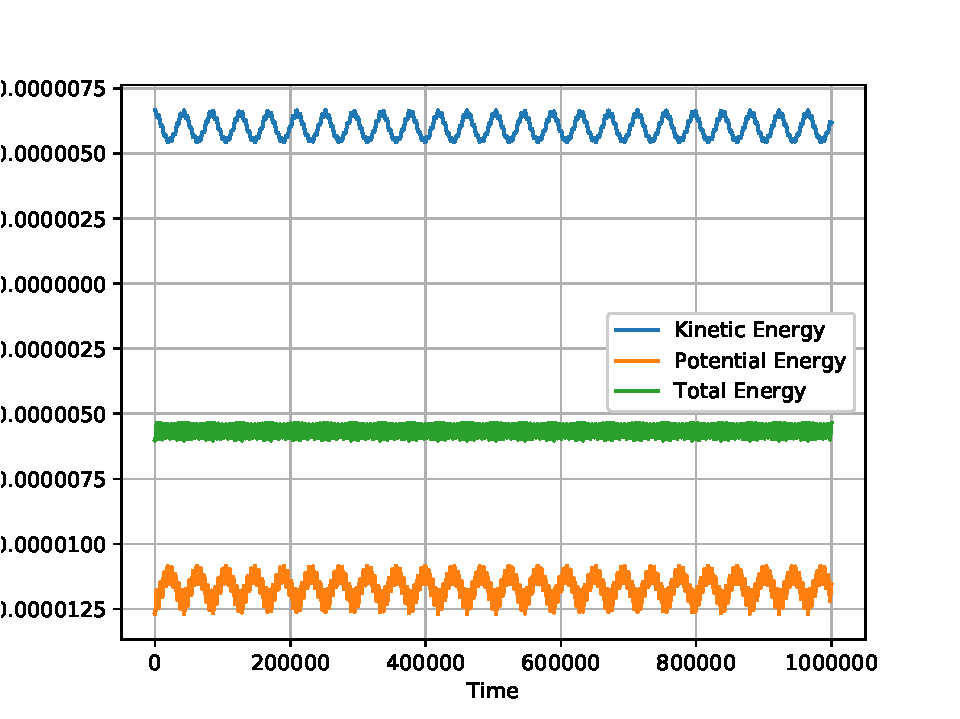
\includegraphics[width=\textwidth]{figures/ast_dumbbell_inertial_energy.pdf}
    \caption{Inertial EOMs energy behavior}\label{fig:inertial_energy}
\end{figure}

\section{Relative Equations of motion}\label{sec:relative_eoms}


\section{Appendix}
